\PassOptionsToPackage{round}{natbib}
\documentclass{tufte-handout}

%\geometry{showframe}% for debugging purposes -- displays the margins
\setcounter{secnumdepth}{3}

\usepackage{amsmath}

% Set up the images/graphics package
\usepackage{graphicx}
\setkeys{Gin}{width=\linewidth,totalheight=\textheight,keepaspectratio}
\graphicspath{{graphics/}}

\title{Research Statement}
\author{D.~Hudson Smith (dane2@clemson.edu)}
%\date{16 January 2024}  % if the \date{} command is left out, the current date will be used

% The following package makes prettier tables.  We're all about the bling!
\usepackage{booktabs}

% The units package provides nice, non-stacked fractions and better spacing
% for units.
\usepackage{units}

% The fancyvrb package lets us customize the formatting of verbatim
% environments.  We use a slightly smaller font.
\usepackage{fancyvrb}
\fvset{fontsize=\normalsize}

% Small sections of multiple columns
\usepackage{multicol}

% Provides paragraphs of dummy text
\usepackage{lipsum}

% These commands are used to pretty-print LaTeX commands
\newcommand{\doccmd}[1]{\texttt{\textbackslash#1}}% command name -- adds backslash automatically
\newcommand{\docopt}[1]{\ensuremath{\langle}\textrm{\textit{#1}}\ensuremath{\rangle}}% optional command argument
\newcommand{\docarg}[1]{\textrm{\textit{#1}}}% (required) command argument
\newenvironment{docspec}{\begin{quote}\noindent}{\end{quote}}% command specification environment
\newcommand{\docenv}[1]{\textsf{#1}}% environment name
\newcommand{\docpkg}[1]{\texttt{#1}}% package name
\newcommand{\doccls}[1]{\texttt{#1}}% document class name
\newcommand{\docclsopt}[1]{\texttt{#1}}% document class option name

\begin{document}

\maketitle% this prints the handout title, author, and date

\begin{abstract}
  \noindent I develop techniques for incorporating prior knowledge into machine learning systems for data-constrained applications. This synthesis of established domain knowledge with flexible machine learning methods leads to better anomaly detection rates, improved sample efficiency, and explainable inference, without sacrificing the expressive power of data-driven techniques like deep learning.
\end{abstract}

%\printclassoptions
\marginnote[1cm]{
  Outline:
  \begin{enumerate}
    \item Research vision
    \item Background
          \begin{enumerate}
            \item Physics
            \item Machine Learning
          \end{enumerate}
    \item Bridging the gap
          \begin{enumerate}
            \item Amortized variational inference
            \item Neural architecture design
          \end{enumerate}
    \item Outlook
  \end{enumerate}
}

\section{Research Vision}
Machine Learning (ML) techniques centered around deep learning and unstructured data are spreading through industry sectors with the promise of solving problems as diverse as drug discovery, personalized medicine, actually helpful AI assistants, generative design, and autonomous driving. In academia, the creation of ML funding mechanisms and the growing volume of ML publications across domains suggest a similar sense of opportunity. In reality, however, there is often a gap between established research methods and the affordances of deep learning (see Table \ref{tab:bigpicture}).

In short, standard deep learning workflows do not naturally incorporate the strong inductive priors often available within problem domains. This gap stymies efforts to make progress on in-domain research using deep learning despite its great potential. {\bf My research aims to bridge this gap, allowing researchers to integrate deep learning into broader projects of discovery.}

\begin{margintable}
  \centering
  \fontfamily{ppl}\selectfont
  \begin{tabular}{ll}
    \toprule
    Deep learning & Established methods \\
    \midrule
    data first    & first principles    \\
    weak priors   & strong priors       \\
    data hungry   & sample efficient    \\
    hands off     & hands on            \\
    flexible      & rigid               \\
    complex       & parsimonious        \\
    opaque        & interpretable       \\
    \bottomrule                         \\
  \end{tabular}
  \caption{Contrasting the general characteristics of deep learning with those of traditional methods used in scientific inquiry.}
  \label{tab:bigpicture}
\end{margintable}

\section{Background}
As a physicist, I learned the power of approaching problems from first principles. As a machine learning scientist, I have seen the power of flexible, data-driven models. This dual experience allows me to integrate the strengths of both approaches.

\subsection{Physics}
My PhD thesis in theoretical physics focused on the quantum behaviors of systems of ultracold atoms. This research relied on a wide range of methods including quantum effective field theory  \citep{smith2015inducing}, computer simulation of interacting quantum systems \citep{langmack2012avalanche}, solutions of systems of differential equations \citep{braaten2014born}, and evolutionary optimization \citep{smith2019engineering}. {\bf In each of these works, I constructed theoretically principled models describing quantum phenomena and calibrated these models to observational data.}

\subsection{Machine Learning}

\begin{marginfigure}%
  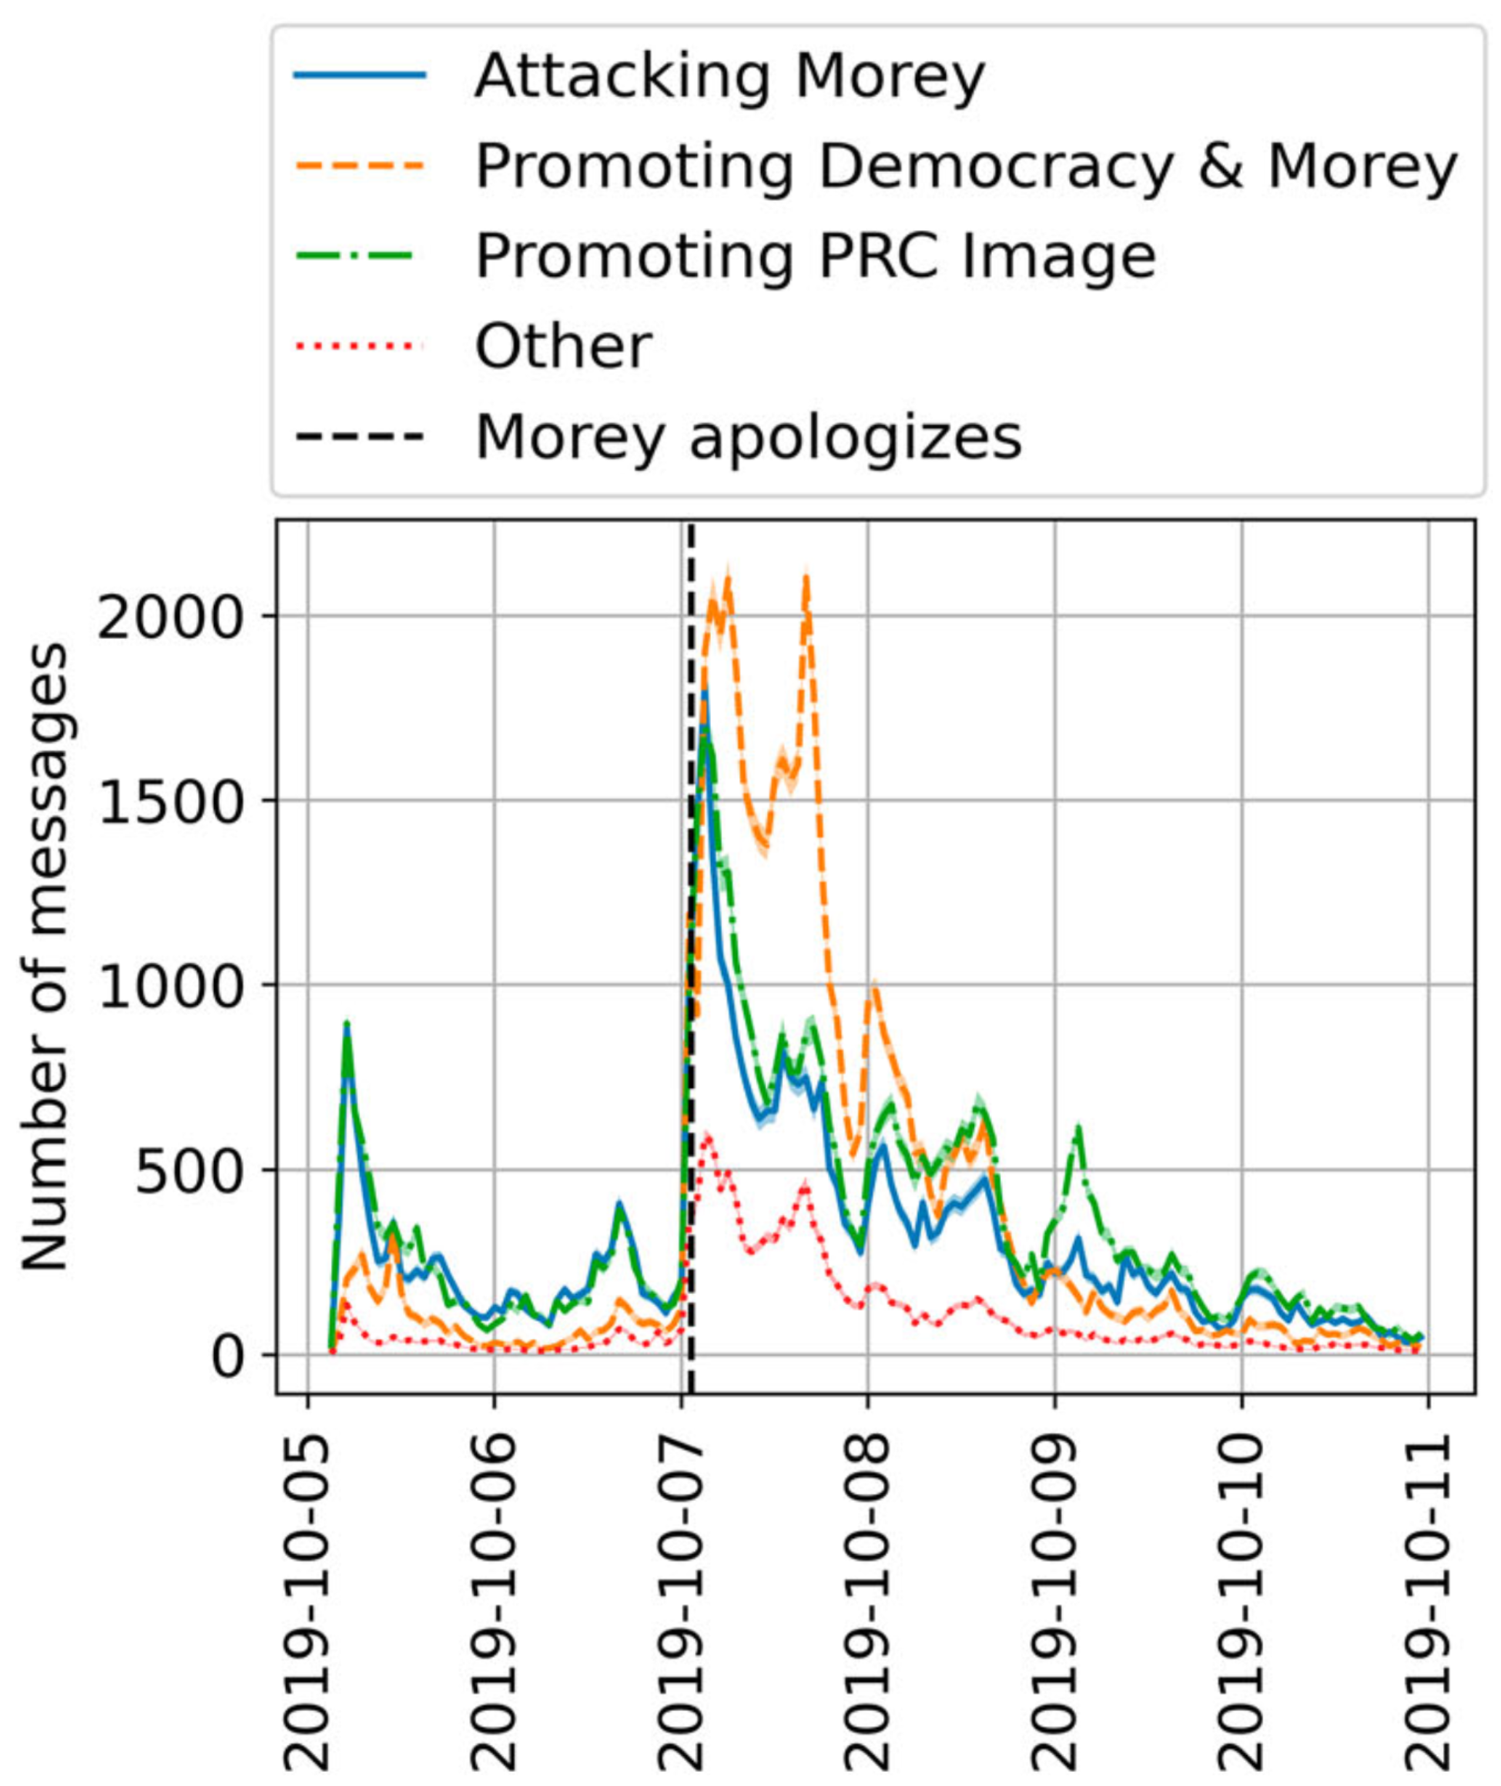
\includegraphics[width=\linewidth]{morey}
  \caption{NLP-driven analysis of the Chinese social media influence campaign centered around the Daryl Morey NBA incident. We use a transformer-based NLP classification architecture to identify each message topic.}
  \label{fig:morey}
\end{marginfigure}

\paragraph{Natural Language Processing (NLP).} In my roles at Clemson, I have interacted with many faculty who would like to automate the analysis of large corpora of textual data. In some cases, the analysis has fit a standard ML workflow. For example, I have collaborated on projects in political science \citep{fine2019content} and communications \citep{ehrett_2021_sscr,cranmer2023social} to automatically label millions of documents via standard NLP classification techniques. These large labeled datasets can then be analyzed to understand how the content relates to other relevant information about the system – e.g., to understand topical trends through time (See Figure \ref{fig:morey}). Other problems do not fit standard ML workflows. For example, how can we use NLP to detect tiny groups of social media accounts participating in Coordinated Information Operations (CIOs)? {\bf Supervised techniques do not apply because the group characteristics are {\it a priori} unknown. Unsupervised anomaly detection fails to distinguish authentic from inauthentic groups. How can we leverage principled knowledge about CIO behavior to isolate inauthentic accounts?} In Section~\ref{sec:avi}, I present a technique that bridges this gap leading to dramatic improvements in the ability to catch the inauthentic accounts.

\begin{marginfigure}%
  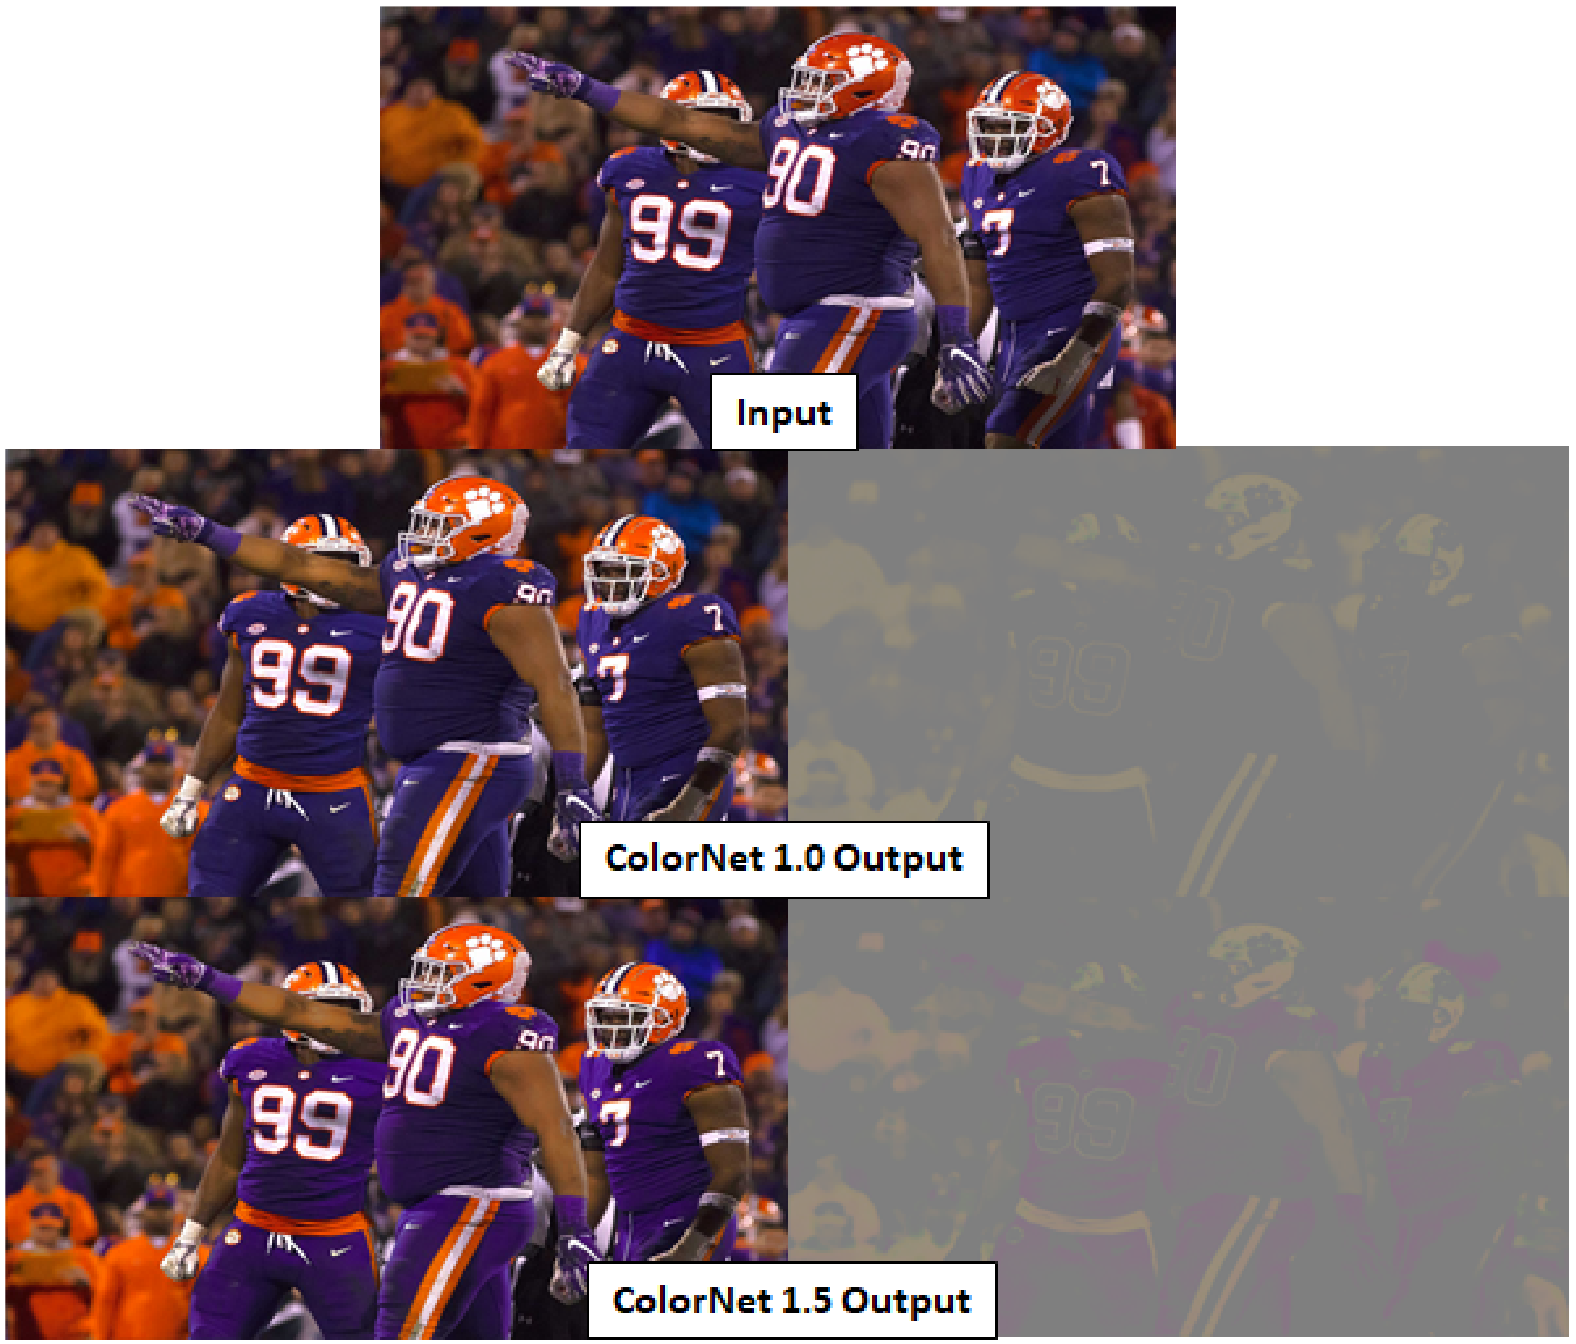
\includegraphics[width=\linewidth]{colornet}
  \caption{Automatic color correction of Clemson brand colors. The correction masks are generated using a convolutional neural network trained using supervised learning. The network was optimized for real-time, high-definition video feeds.}
  \label{fig:colornet}
\end{marginfigure}

\paragraph{Computer Vision.} Some computer vision problems fit into standard ML workflows. For example, my colleagues and I successfully applied deep learning techniques to classify the health state of plants under various environmental stresses \citep{freeman2019watson}, to automatically correct brand color representation in broadcast footage \citep{mayes_2021_smpte} (See Figure \ref{fig:colornet}), and to detect the image quality of ultrasound exam images \citep{taye2022deep}. As with text, however, many compelling questions do not fall neatly within the traditional workflows. For example, in collaboration with physicians at MUSC, I am working on automatically detecting congenital heart defects from infant ultrasound videos. The supervisory signal is highly sparse: one binary outcome per video. {\bf Using standard deep learning algorithms, this sparsity would necessitate access to a prohibitively large labeled set of videos. How can we leverage inductive priors related to the nature of the relevant signal to mitigate this sparsity?} In Section~\ref{sec:usvn}, I present my work incorporating these priors into a deep learning architecture to dramatically improve sample efficiency and model interpretability.

\section{Bridging the gap}\label{sec:current}

\subsection{Amortized variational inference}\label{sec:avi}
Amortized variational inference (AVI) is a flavor of variational Bayesian inference that models parametric posterior and generative distributions using mappings that are shared among samples. The mapping functions can be deep neural networks. Domain researchers can incorporate inductive priors into the structure of the probabilistic model and the choice of prior distributions for latent random variables while benefiting from the expressiveness of neural networks. {\bf Thus, AVI provides a natural bridge between deep learning techniques and established methods and knowledge.}

In work currently under review\thanks{preprint available at \url{https://arxiv.org/abs/2401.06205}}, my colleagues and I present a method for the unsupervised detection of small coordinated groups of accounts on social media, such as those created by the Russian-backed Internet Research Agency (IRA) surrounding the 2016 US presidential election. Among other results, we demonstrated near-perfect unsupervised detection of the inauthentic accounts that participated in a CIO backed by the Chinese Communist Party (CCP) targeting Western sentiment toward CCP activities in the Xinjiang province (See Figure \ref{fig:trolls}). Without further manual tuning, this approach showed strong detection performance for four distinct CIOs backed by different actors and targeting different audiences.

\begin{marginfigure}
  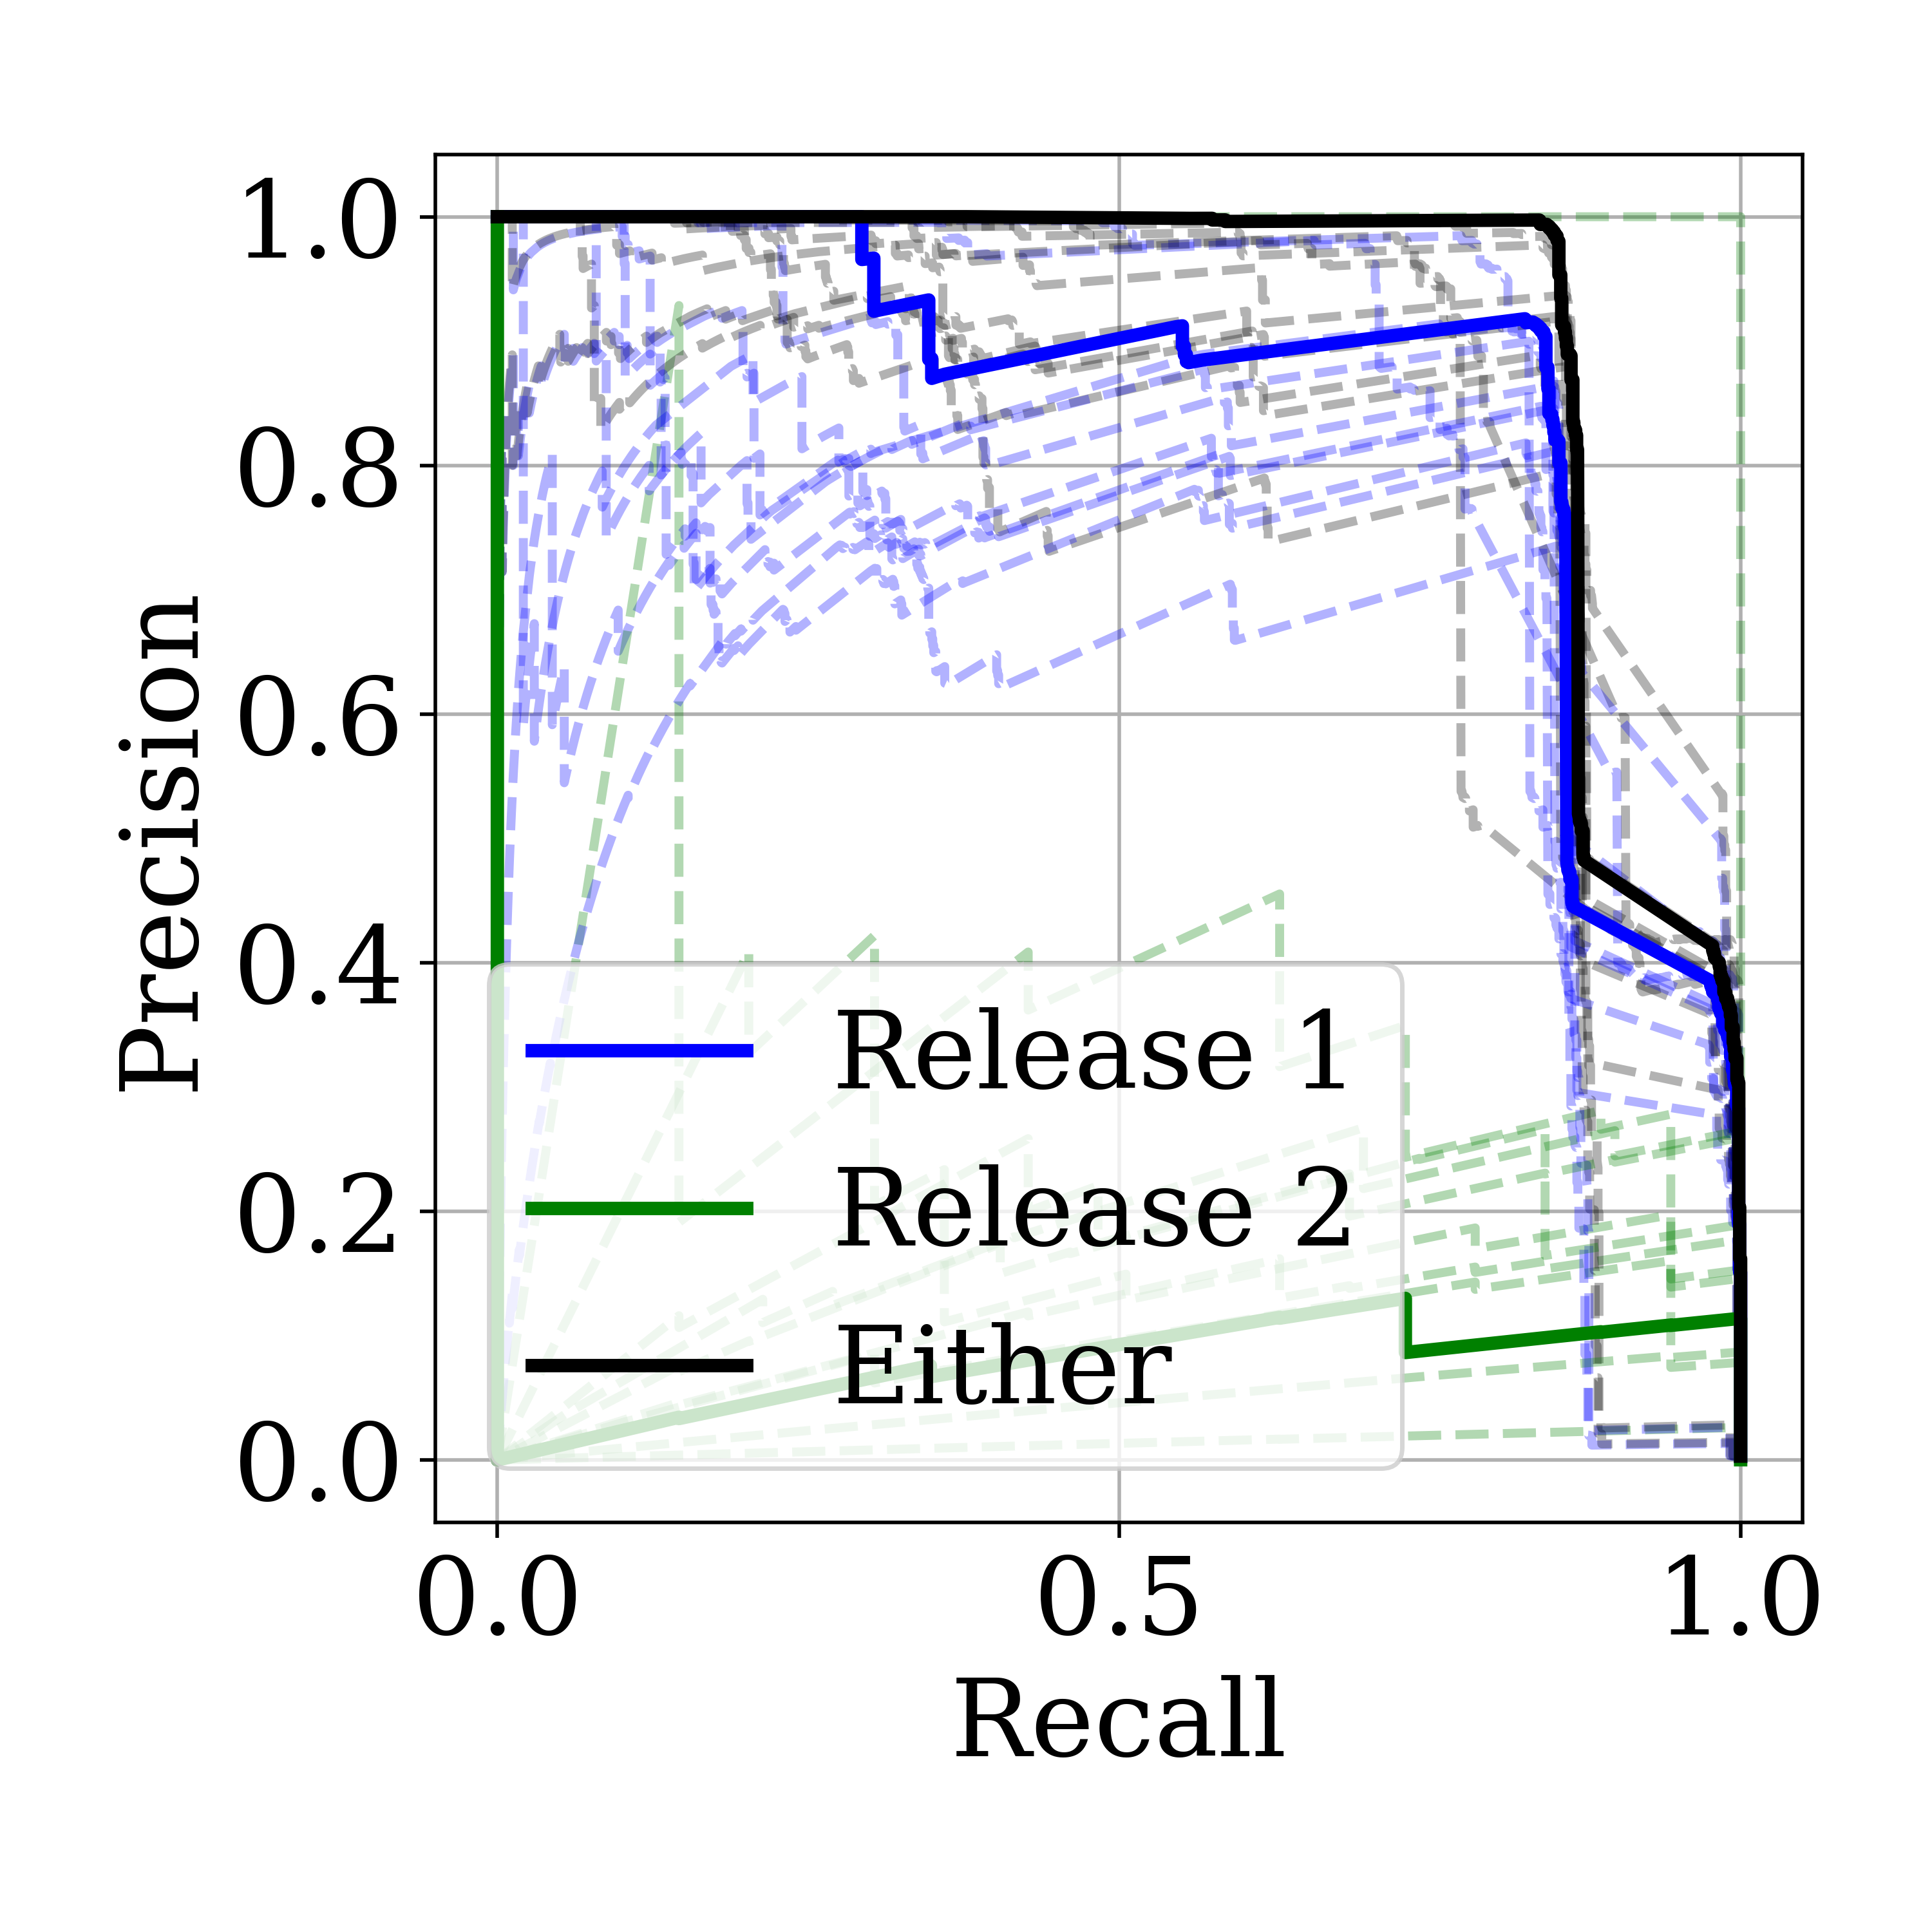
\includegraphics[width=\linewidth]{precrec_xj}
  \caption{Detection curves for accounts involved with the CCP-backed Xinjiang CIO. This CIO consisted of two groups of coordinating accounts that operated according to slightly different strategies. We evaluate the detection performance for these separately (Release 1 and 2) or together (Either). The area under the precision-recall curve for detecting Either is 90\%, representing a 300-fold improvement relative to a random-search baseline.}
  \label{fig:trolls}
\end{marginfigure}

I am now working to apply these techniques to medical computer vision problems where labeled data is costly, but many things are known {\it a priori} about the relevant visual characteristics in the imagery. For instance, when identifying congenital heart defects in ultrasound imagery, the relevant visual information is contained in small connected regions. Standard deep learning networks would need to learn this fact from the data, thereby requiring larger numbers of samples. I am leveraging this insight using AVI and Gaussian Markov Random Field priors to improve sample efficiency.

\subsection{Neural architecture design}\label{sec:usvn}
Inductive priors can be built into deep-learning network architectures. The now famous convolutional neural network (CNN) architecture builds in translational invariance of features in the image plane. This assumption reduces the data and compute resources needed to train effective image processing networks. {\bf Similarly, many applications could benefit from converting in-domain knowledge into the network architecture.}

Working closely with collaborators at MUSC and Prisma Health, I observed that many ultrasound video analysis tasks can be modeled using the assumption of temporal independence. This is because the subject of the video (the anatomy) is often static, with all dynamics driven by the sonographer with the goal of locating the relevant anatomical view. Based on this insight, I developed the Ultrasound Video Network (USVN), which adaptively pools information from different frames in a time-invariant manner using an attention mechanism \citep{smith2023relevance}. The resulting network performs significantly better than state-of-the-art video networks on detecting {\it Patent Ductus Arteriosus} (PDA) and in assessing the diagnostic quality of Focused Assessment with Sonography for Trauma (FAST) exam videos, especially when artificially limiting the amount of training data.

\begin{marginfigure}
  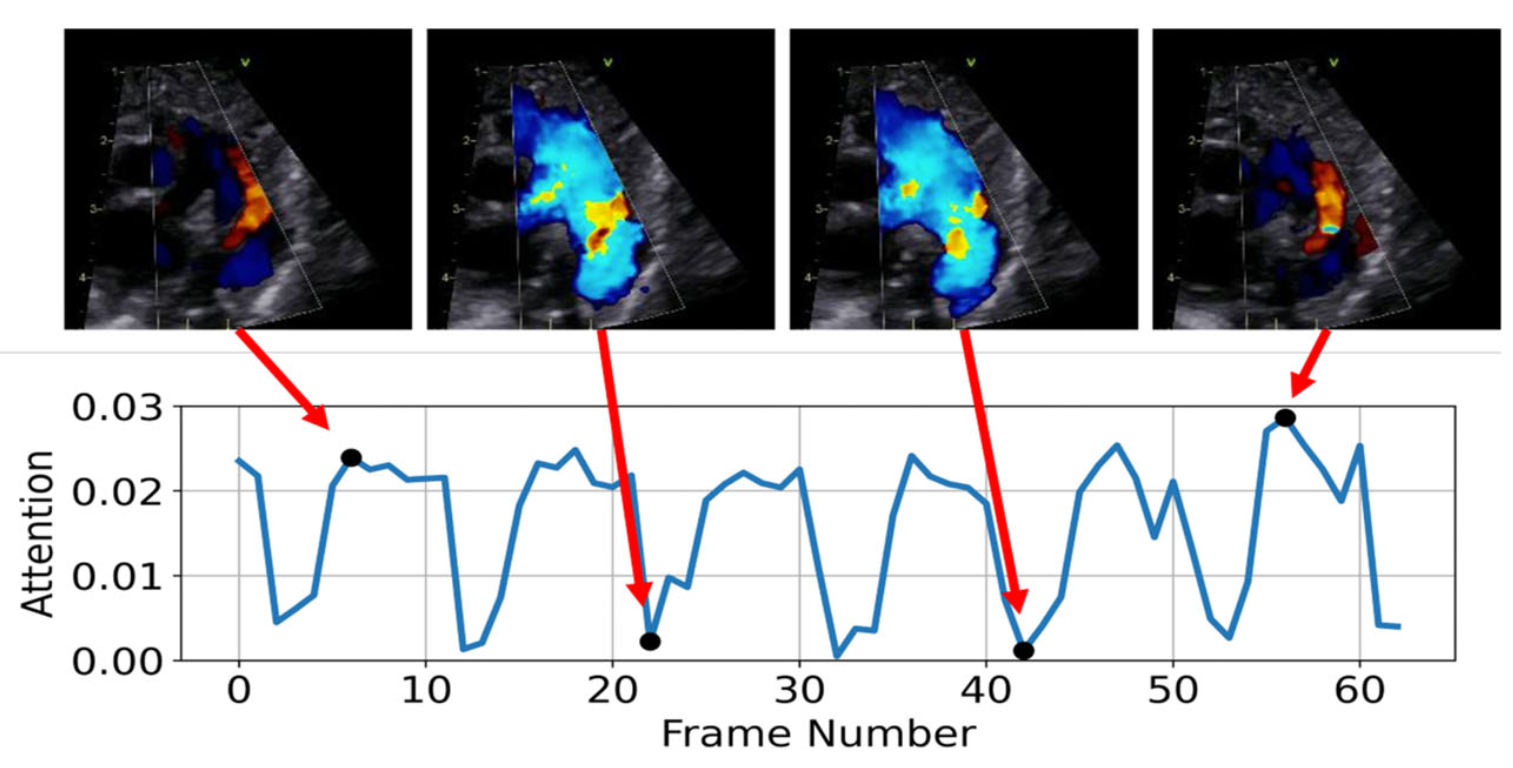
\includegraphics[width=\linewidth]{attn}
  \caption{The attention weights are high at the relevant parts of the cardiac cycle for PDA detection. The PDA is visible as the concentrated red region in the high-attention frames.}
  \label{fig:attn}
\end{marginfigure}
The assumption of temporal independence also improves model interpretability. The attention mechanism computes a weighting factor for each frame. Clinicians can interpret these weights as the relevance of the frame for the recognition task by aligning the weights with the content of the frames, as shown in Figure \ref{fig:attn}. In the case of PDA detection, the attention scores correlate with the cardiac cycle, with high attention given to the parts of the cycle that reveal the PDA.

\section{Outlook}
My upcoming work further develops and validates techniques that enable domain researchers to augment their existing methods with deep learning to solve new problems. Soon, I plan to extend the methods I described above to new areas. For example, I am now working on using AVI to build spatial sparsity priors into deep-learning models to improve sample efficiency for image tasks. Following that, I plan to explore using shape priors with deep learning to encode even richer information about the problem domain. I am also exploring the integration of AVI and architecture design. For example, in some ultrasound recognition tasks, only a tiny fraction of video frames contain relevant information. The USVN attention mechanism described in \ref{sec:usvn} can be extended to encode this sparsity by treating the attention weights as a latent random variable with a sparsity-inducing prior distribution.

In addition to AVI and architecture design, network pretraining techniques provide a third way to incorporate domain knowledge into a deep learning application. Working with a Biomedical Datascience and Informatics PhD student, I am exploring ways to integrate medical-specific knowledge into pretrained image representation networks for better performance on medical tasks. Such an advance would improve sample efficiency across many medical image analysis tasks at once with many benefits to the medical imaging community.

To fund this research, I intend to submit an NIH K25 Mentored Quantitative Research Development Award\thanks{\url{https://grants.nih.gov/grants/guide/pa-files/PA-20-199.html}} which is explicitly designed for "those investigators whose quantitative science and engineering research has thus far not been focused primarily on questions of health and disease." I am also considering submitting an NSF Career award with a stronger focus on the methodological aspect of my work. These awards can build upon my current work funded through the NIH COBRE program.


\bibliography{../pubs}
\bibliographystyle{plainnat}



\end{document}
